\chapter{\glsentrylongsp{ci}}
\label{ch:sota-ci}

El comportamiento de un individuo en un entorno se ve influenciado por una infinidad de variables. Identificar las relaciones entre éstas es en la mayoría de las ocasiones una tarea que va de lo muy difícil a lo imposible, más aún si añadimos que éstas son muy numerosas y pueden llegar a ser imposibles de cuantificar o incluso de detectar.

La \ac{ci} engloba un conjunto de técnicas que facilitan enormemente estas tareas. En este capítulo se ofrece una perspectiva de la literatura actual sobre las técnicas de la \gls{ci} que son de interés para esta tesis. Introduciremos el concepto y las nociones de \enquote{agente} y de \enquote{aprendizaje} para posteriormente introducir algunas de las técnicas utilizadas dentro del área. Por último, desarrollaremos en detalle las dos técnicas técnicas principales sobre las que se apoya el trabajo teórico de esta tesis: \glsentrylongplsp{ann} y \glsentrylongsp{fl}.

\section{\glsentrylongsp{ai} vs. \glsentrylongsp{ci}}

¿Qué es la \ac{ci}? Para entender el significado de éste término tenemos que entender cómo ha evolucionado el término \ac{ai} a lo largo de los años.

El primer concepto a introducir es el de \textbf{conexionismo}. Se puede considerar a Santiago Ramón y Cajal como principal precursor de esta idea por sus trabajos acerca de la estructura de las neuronas y sus conexiónes (e.g. \cite{y1888estructura} y~\cite{ramon1904textura}). Otros prefieren citar el trabajo \textit{\enquote{A logical calculus of the ideas immanent in nervous activity}} (\cite{McCulloch1943}) sobre \glspl{ann} o \textit{\enquote{The organization of behavior}} (\cite{hebb19680}) acerca de la teoría del aprendizaje como primeros trabajos en este tema. Independientemente de su origen, el conexionismo postula que tanto la \textit{mente} como el \textit{conocimiento} emergen de redes formadas por unidades sencillas interconectadas (i.e. neuronas).

\marginnote{
	\textbf{El Test de Turing} es un modelo que propuso Alan Turing para probar si una máquina es capaz de exhibir comportamiento inteligente similar al del ser humano. Hay tres participantes, dos humanos ($A$ y $C$) y una máquina ($B$), separados entre sí pero pudiendo intercambiarse mensajes de texto. $C$ envía preguntas a $A$ y $B$ sin saber quién es humano y quién es máquina y éstos le responden. Si $C$ no es capaz de identificar qué participante es la máquina, se puede concluir que la máquina es inteligente.
}

Por otro lado, en 1950, Alan Turing publicó un artículo que comenzaba con la frase \textit{\enquote{Can machines think?~\cite{turing1950computing}}}\sidenote{
	El concepto de \enquote{pensar} es en sí un tema controvertido en el propio ser humano: ¿pensar es algo inherentemente biológico? ¿surge de la mente? Tanto si sí como si no, ¿de qué forma lo hace? Por ello existen detractores de la validez del Test de Turing como, por ejemplo, el experimento de la habitación china, propuesto por John Searle.
	
	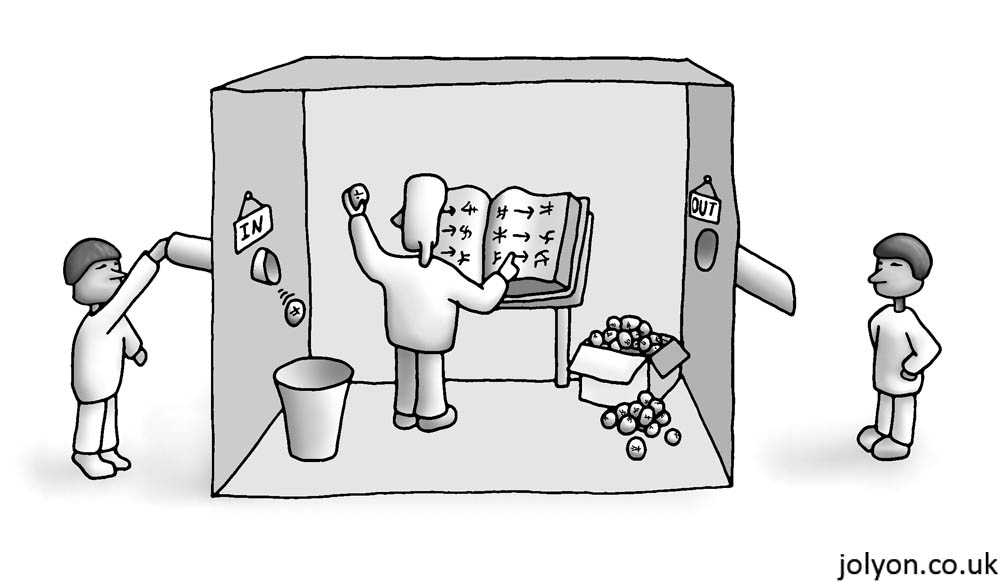
\includegraphics{chinese-room}
	
	Se parte de un Test de Turing donde la máquina ha aprendido a hablar chino. Se reemplaza por una persona que no sabe nada del idioma pero que va equipada con un manual de correspondencias de ideogramas. Cuando una persona le manda mensajes en chino, esta otra responde. Evidentemente la persona no sabe hablar chino, y por ello no podemos afirmar que la máquina sabe hablarlo. Sin embargo, esto lleva a cuestiones quizá más intrigantes. Por ejemplo, si la máquina es capaz de realizar una acción sin entender lo que hace y por qué lo hace, ¿qué garantías tenemos de que el humano sí es capaz? Si los ordenadores operan sobre símbolos sin comprender el verdadero contenido de éstos, ¿hasta qué punto los humanos lo hacen de forma diferente?.
}, introduciendo el famoso Test de Turing para determinar si una máquina es o no inteligente. Se puede considerar este momento como el punto donde se estableció el objetivo a largo plazo del campo de la \ac{ai}, ya que en el artículo Turing propuso un método para determinar si una máquina era capaz de exhibir comportamiento inteligente. Sin embargo, no fue hasta $1956$ en la Conferencia de Dartmouth~\cite{mccarthy1956dartmouth} donde John McCarthy acuñó el término~\ac{ai} a la vez que presentó el tema de la conferencia como la pregunta realizada por Turing en dicho artículo.

A partir de este punto la investigación en~\ac{ai} recibió muchísima atención por parte de investigadores y gobiernos, lo que se tradujo en financiación. Los estudios estaban dominados por aquellos relacionados con las ideas del conexionismo hasta que en $1969$, se publicó el libro \textit{Perceptrons}~\cite{minsky1969perceptrons} de Marvin Minsky y Seymour Papert, donde se expusieron las limitaciones de los modelos de \acp{ann} desarrollados hasta la fecha. El impacto fue tal que la investigación en \gls{ai} se abandonó casi por completo. Concretamente el conexionismo dejó de estar presente en la literatura científica durante dos décadas. Es lo que se conoce como el primer \textit{AI Winter}.

\marginnote{
	\textbf{El AI Winter} no sólo se produjo por el efecto gurú del libro \textit{Perceptrons}, aunque éste fue la gota que colmó el vaso. A la emoción inicial por los avances le siguieron muchos años de promesas incumplidas, investigación sin resultados significativos, limitaciones de hardware, aumento de la complejidad del software (los comienzos de la crisis del software \cite{dijkstra1972humble}). Todo ello provocó un desinterés y una disminución de la financiación que se retroalimentaron la una a la otra.
}

El interés por el campo volvió de nuevo a principios de los $80$ con la aparición en escena de los primeros \glsentrylongplsp{esys}, los cuales se consideran como el primer caso de éxito en la \gls{ai} (\cite{russell2003artificial}). A finales de la década, sin embargo, empezaron a resurgir los enfoques conexionistas, en gran parte por la aparición de nuevas técnicas de entrenamiento en perceptrones multicapa y por el concepto de activación no lineal en neuronas \cite{rumelhart1985learning, cybenko1989approximation}). En este momento los sistemas expertos empezaron a perder interés frente al nuevo avance del conexionismo. Ésta década es conocida como segundo \textit{AI Winter} dado que la investigación sobre \glsentrylongplsp{esys} disminuye. Sin embargo no fue un abandono tan acusado como el del primero.

Mientras que el enfoque clásico de la \gls{ai} postulaba que la mente opera de la misma manera que una máquina de Turing, es decir, mediante operaciones sobre un lenguaje de símbolos, el enfoque del conexionismo postula que la mente, el comportamiento inteligente, emerge de modelos a más bajo nivel. Esto provocó que algunas voces se alzaran contra lo que se consideraba el \textit{enfoque incorrecto} de la \gls{ai}. Después de todo, los modelos desarrollados en los métodos clásicos son fáciles de interpretar mientas que los del enfoque conexionista no son del todo deducibles, más aún si estos problemas son de naturaleza estocástica.

Sin embargo, otras técnicas alineadas con el conexionismo como la \glsentrylongsp{fl} o los \glsentrylongplsp{ga} ganaban popularidad y alimentaban el éxito del nuevo enfoque. Esto provocó una explosión de terminologías para diferenciar las investigaciones de la propia~\ac{ai} clásica. Por un lado se evitaba el conflicto, nombrando las áreas de trabajo con un término más acorde con el comportamiento o técnica utilizada. Por otro, se separaba de las connotaciones negativas que fue cosechando la \ac{ai} con el paso de los años (i.e. promesas, pero no resultados).

Lo verdaderamente interesante es ver la evolución de la literatura, y por tanto de los objetivos de la \ac{ai} durante estos años. En el nacimiento del campo, se buscan literalmente máquinas que piensen como humanos, o al menos seres racionales, con mente. Con el paso de los años (y los continuos choques contra la realidad), la literatura va tendiendo hacia la búsqueda de conductas y comportamientos inteligentes cada vez más específicos. Este hecho se hace más patente en este momento, donde cada investigación se nombra de cualquier forma menos con el término \ac{ai} (e.g \ac{ml}, \acp{rs}, o \ac{nlp}). Es evidente que la \ac{ai} se puede observar desde diferentes puntos de vista, todos perfectamente válidos. En~\cite{russell2003artificial}, tras un análisis de las definiciones existentes en la literatura por parte de diferentes autores, se hace énfasis en este hecho mostrando los diferentes puntos de vista a la hora de hablar de lo que es la \ac{ai}. El resumen se puede observar en la figura~\ref{fig:different-povs-ai}.

Volviendo al tema de la terminología, muchas de las técnicas se fueron agrupando dentro de diferentes áreas. Una de ellas es la conocida como \glsentrylongsp{ci}. Dado que persigue el mismo objetivo a largo plazo y que surje de la propia \ac{ai} parece lógico mantenerla como un subconjunto y no como un nuevo campo del conocimiento humano. Sin embargo, algunos autores abogan por que la \ac{ci} es un campo diferenciado de la \ac{ai}.

Podemos definir la \ac{ci} como la \enquote{\textit{rama de la \ac{ai} que aporta soluciones a \textbf{tareas específicas} de forma \textbf{inteligente} a partir del aprendizaje mediante el uso de \textbf{datos experimentales}}}. A diferencia de la aproximación clásica de la \ac{ai}, se buscan aproximaciones a las soluciones y no las soluciones exactas. Esto es debido a que muchos problemas son de naturaleza compleja, ya sea por la erlación entre sus multiplas variables, a la falta de información o a la imposibilidad de traducirlos a lenguaje binario.

\begin{figure}
	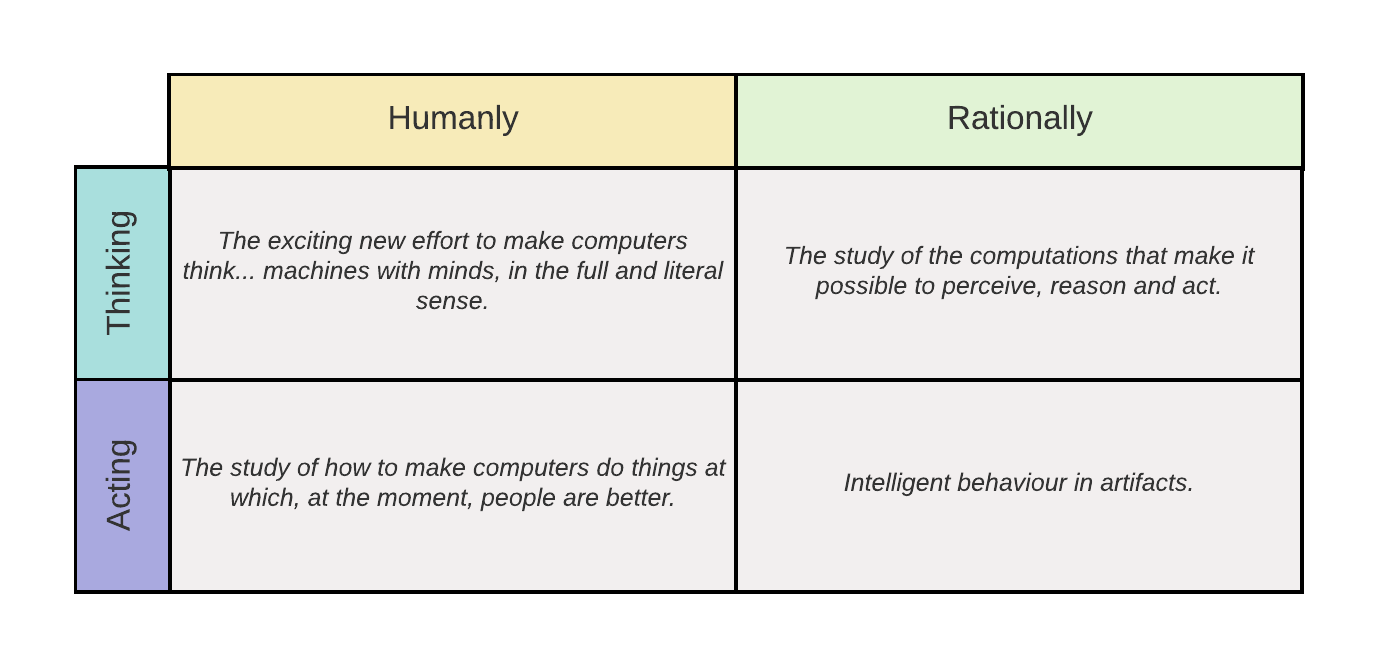
\includegraphics{different-povs-ai}
	\caption[Diferentes objetivos perseguidos por la \glsentrylongsp{ai}]{Diferentes objetivos perseguidos por la~\glsentrylongsp{ai}. Las filas diferencian entre pensamiento o comportamiento mientras que las columnas separan entre inteligencia humana o el ideal de la inteligencia (racionalidad). Fuente: \textit{Artificial Intelligence: A Modern Approach ($3^{rd}$ Ed.)},~\cite{russell2003artificial}.}
	\label{fig:different-povs-ai}
\end{figure}

Se puede establecer el año $1994$ como en el que la \glsentrylongplsp{ci} nace formalmente como área, coincidiendo con el cambio de nombre del \textit{IEEE Neural Networks Council} a \textit{IEEE Computational Intelligence Society}\sidenote{
	\url{http://cis.ieee.org/}
}. Poco antes, en $1993$, Bob Marks presentaba las que él consideraba diferencias fundamentales entre la \glsentrylongsp{ai} clásica y la \glsentrylongsp{ci}, resumiéndolas en la siguiente frase:

\blockquote{Neural networks, genetic algorithms, fuzzy systems, evolutionary programming, and artificial life are the building blocks of CI.}

Durante estos años ganaba popularidad también el concepto del \gls{sc} en contraposición con el \gls{hc}. El \gls{sc} engloba las técnicas que buscan resolver problemas con información incompleta o con ruido. Debido a que el conjunto de técnicas definidas como consituyentes del \gls{sc} son las mismas que se usan en la \gls{ci} algunos autores consideran ambos términos equivalentes. Nosotros consideramos que el \gls{sc} es un punto de vista de la computación y que la \gls{ci} es un área de la \glsentrylong{ai} hace uso de métodos del \gls{sc}.

\marginnote{
	\textbf{\gls{hc} y \gls{sc}} son la forma de referirse a la computación convencional frente al \gls{sc}. El \gls{hc} basa sus técnicas en aquellas basadas en modelos analíticos definidos de forma precisa y que en ocasiones requieren mucho tiempo de cómputo. Están basados en lógica binaria, análisis numérico, algoritmos y respuestas exactas. El \gls{sc} por otro lado es tolerante a la imprecisión y al ruido y tiende a llegar a soluciones aproximadas de manera más rápida. Se basa en modelos aproximados, emergencia de algoritmos y modelos estocásticos.
}

\section{Aprendizaje}

\TODO{Fusionar los dos párrafos siguientes y el de la margin note con el párrafo anterior y crear una nueva introducción para la parte del aprendizaje. Sobre todo hacer hincapié en que en el HC lo normal es desarrollar una solución para el problema en cuestión mientras que en el Soft Computing lo normal es tener un modelo que se tunea y/o que aprende a solucionar un problema determinado.}

La resolución clásica a un problema suele ser la aplicación de una secuencia de instrucciones basadas en un conjunto de símbolos (e.g. una función escrita en el lenguaje de programación C). Esta forma de solucionar un problema no \textit{aprende} a solucionarlo. Se puede interpretar como que la solución está grabada en su memoria.

En la aproximación de la \gls{ci}, existen modelos y existen técnicas para hacer aprender esos modelos. La aplicación de dichas técnicas es lo que se conoce como \textbf{aprendizaje}. Las técnicas de aprendizaje en \gls{ci} se suelen clasificar en $3$ paradigmas:

\begin{itemize}
	\item \textbf{Supervisado}. El entorno presentado al modelo consiste en un conjunto de la forma $D = {(I_i, O_i) | \forall i \in \mathbb{N}}$, donde cada $O_i$ es la salida esperada del modelo a la entrada $I_i$. Los algoritmos tratarán de ajustar el modelo todo lo posible para que las salidas obtenidas sean lo más parecidas a las salidas originales. Este paradigma de entrenamiento suele estar relacionado con problemas de \textit{regresión}.
	\item \textbf{No supervisado}. Al modelo se le ofrece un conjunto de la forma $D = {I_i | \forall i \in \mathbb{N}}$, donde cada $I_i$ es una entrada al problema, pero del que no conocemos la salida. Los algoritmos dentro de esta categoría harán uso de estos datos para ir reajustando el modelo tratando de encontrar las estructuras ocultas entre dichos datos (e.g. patrones, correlaciones o clases). Es un paradigma de entrenamiento íntimamente relacionado con problemas de \textit{clasificación}.
	\item \textbf{Por refuerzo}. \TODO{Explicar}
\end{itemize}

Algunos autores hacen uso de técnicas pertenecientes a ambos paradigmas en forma de aproximación híbrida para suplir deficiencias u optimizar/acelerar el aprendizaje. Un claro ejemplo lo podemos ver en \cite{Hinton2006}, donde los autores hacen uso de \textit{autoencoders} como técnica no supervisada para la inicialización de los pesos de una red neuronal y posteriormente realizan un entrenamiento supervisado para la optimización es éstos.

\section{Técnicas en la \Glsentrylongsp{ci}}

Bajo el paraguas de la \ac{ci} se incluyen muchas técnicas diferentes, entre las cuales están las usadas en esta tesis. El resto de la sección describe el funcionamiento de cada una de estas técnicas. \TODO{Reescribir esto porque parece que lo ha escrito un crío de la ESO}

\subsection{\Glsentrylongplsp{ann}}

Son herramientas que tratan de replicar las funciones cerebrales de un ser vivo de una manera muy fundamental, esto es, desde sus componentes más básicos, las neuronas. Para ello se basan en estudios de neurobiología y de ciencia cognitiva moderna del cerebro humano\sidenote{
	Aún apoyándose en la topología y funcionamiento del cerebro humano para realizar el símil, lo cierto es que dichos modelos distan aún de considerarse \textit{cerebros artificiales}. La red neuronal más compleja hasta la fecha es la propuesta en~\cite{TraskANDREWTRASK}, con alrededor de $160.000$ parámetros a ser ajustados (podemos abstraernos y pensar en ellos como conexiones entre neuronas). Si comparamos esta cifra sólo con las del neocórtex (figura~\ref{fig:neocortex}) hace que, tecnológicamente hablando, nos quedemos con la sensación de estar aún a años luz de aproximarnos a la complejidad de un cerebro humano.
}.

Una \ac{ann} es independiente del problema a solucionar. Se la puede considerar como una caja negra que aprende las relaciones que subyacen en los datos de un problema para abstraer el modelo a partir de éstos. Estas características de aprendizaje y abstracción son los factores determinantes por los que son usadas en prácticamente todas las áreas de la ciencia y de la ingeniería (\cite{Du2006}).

\begin{figure}
	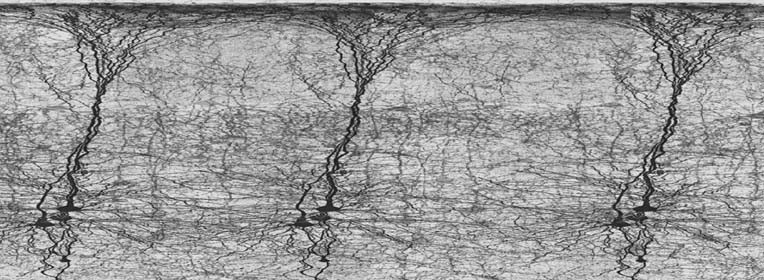
\includegraphics{neocortex}
	\caption[Ilustración de una sección del neocórtex humano]{Sección del neocórtex humano, región asociada a las capacidades cognitivas y que supone alrededor de un $76\%$ del volumen total del cerebro humano. Está distribuído en $6$ capas y miles de columnas que las atraviesan, cada una con alrededor de $10.000$ neuronas y un diámetro de $0.5mm$.  Como dato anecdótico, se estima que sólo en el neocórtex humano existen alrededor de $20.000$ millones de neuronas, cada una de las cuales conectada a entre $100$ y $100.000$ neuronas vecinas (\cite{Pakkenberg1997}). Esto supone entre $2 \cdot 10^{12}$ y $2 \cdot 10^{15}$ conexiones. Fuente: \textit{Blue Brain Project EPFL}, \url{http://bluebrain.epfl.ch/}.}
	\label{fig:neocortex}
\end{figure}

\newthought{El primer trabajo} en la disciplina se le atribuye a  los investigadores McCulloch-Pitts por su modelo de neurona artificial ilustrado en la figura~\ref{fig:mccullocs-pitts-neuron-model} (\cite{McCulloch1943}). Existen diferentes tipologías y formas de operar con redes, pero todas funcionan de la misma manera: unidades (e.g. neuronas) interconectados mediante enlaces por los que fluye la información de manera unidireccional, donde algunas de dichas unidades sirven de entrada al sistema (i.e. entradas o sensores), otras sirven de salida del sistema (i.e. salidas y actuadores) y otras como elementos internos (i.e. ocultas), y donde las conexiones se ajustan mediante un proceso denominado \textit{entrenamiento}.

\begin{figure}
	\missingfigure[figheight=2cm]{Figura del modelo artificial de McCullocs-Pitts}
	\caption[Modelo de neurona artificial de McCulloch y Pitts]{Variación de la representación del modelo de neurona artificial propuesto por McCulloch y Pitts. En éste, cada una de las entradas $x_i$ es incrementada o inhibida aplicando el producto con su peso asociado $w_i$. La activación vendrá determinada por la aplicación de una función (denominada \enquote{de activación}) a la suma de los valores. Esta variación en concreto incluye una entrada $x_0$ y un peso $w_0$ como bias de la neurona para la variación dinámica del umbral de activación.}
	\label{fig:mccullocs-pitts-neuron-model}
\end{figure}

Este primer modelo de neurona proponía una función escalón para determinar si la neurona se activaba o no (analogía al funcionamiento de la neurona artificial). \TODO{Parrafito sobre la limitación de la neurona singular para dar hilo a las topologías}.

Posteriormente aparecieron nuevos modelos de neuronas con diferentes funciones de activación. De éstas, las más comunes son las de tipo sigmoide\sidenote{
	Concretamente la función logística de pendiente $1$ definida como:
	\begin{equation}
		\frac{1}{1 + e^{-x}}
	\end{equation}
}.\TODO{Actualizar esto porque creo que empieza a er ás común la ReLU, que se usa hasta en la sopa. Una o dos ilustraciones mostrando los diferentes tipos (grafiquitas) de las funciones de activación en redes neuronales. Para que sea de un poco más de 1990 y no esta mierad. Poner escalón, sigmoidal y tanh (como clásicas)y ReLU y adjustid ReLU (o como coño se llamen) como modernas.}

\newthought{Existen diferentes topologías de redes neuronales} o arquitecturas dependiendo de qué forma toma el grafo que modela las neuronas y sus conexiones. En este caso, las redes neuronales pueden ser de dos tipos:

\begin{itemize}
	\item \textbf{Feed-Forward}. Sus grafos no contienen ninguń ciclo (figura XXX) |\TODO{Esa pedaaaaaso de figura. A lo mejor hacer una que incluya tres ejemplos.}. Es la topología más usada en aplicaciones prácticas debido a su sencillez y su efectividad. En ellas el flujo de información sigue un camino desde las entradas hasta las salidas, sin ninguna retroalimentación. No es requisito que las neuronas se agrupen en capas, aunque suele ser la estructura común. A las redes de más de dos capas ocultas (i.e. las capas que se encuentran entre la capa de neuronas de entrada y la capa de neuronas de salida) se las denomina \enquote{profundas} o \textit{deep}. Algunos tipos pertenecientes a esta categoría pueden ser el Perceptrón [Rosemblat, 1957], el Perceptrón multicapa [Rumelhart et al., 1986], el algoritmo LVQ y su sucesor los Mapas Auto-Organizados [Kohonen, 1998].
	\item \textbf{Recurrentes}. Sus grafos contienen uno o más ciclos, de tal manera que el flujo de información de salida de una neurona puede llegar a afectar a su propio estado. Estas topologías representan de una forma más fiel las bases biológicas de las \ac{ann}, pero son más complejas a la hora de operar y entrenar. Algunos casos particulares de este tipo de arquitectura son las Redes de Hopfield [Hopfield, 1982] o las memorias LSTM (del inglés Long-Short Term Memory) [Hochreiter \& Schmidhuber, 1997].
\end{itemize}

\TODO{Desarrollar un poquito el tema de los grafos computacionales indicando que si bien no se tratan de una técnica dentro de la inteligencia computacional, sí que se usan para representar operaciones.}

\subsection{Grafos computacionales}

En la actualidad el concepto de grafo computacional se relaciona directamente con las redes neuronales, y por ello se introduce el concepto en este apartado. Sin embargo, no se trata de un concepto exclusivo de esta técnica. De hecho, ni siquiera es un concepto perteneciente al área de la inteligencia computacional, sino que es simplemente una forma de representar operaciones sobre datos.

Formalmente, un \textbf{grafo computacional} es un grafo dirigido donde los vértices representan operaciones sobre datos mientras que las aristas representan el flujo de dichos datos. La figura XXX ilustra un ejemplo de un grafo computacional.

Una ventaja al representar un modelo como grafo computacional es que ayuda a abstraerse de la formas de las entradas y las salidas, facilitando el trabajo de operaciones en batch. Otra ventaja, todavía mayor, es que, al organizar de entrada a salida (en la figura XXX de izquierda a derecha) las operaciones que se necesitan para obtener una salida a partir de una entrada, en los casos donde el objetivo es optimizar la salida permiten fácilmente representar el gradiente al organizarlo del modo contrario (es decir, de las salidas a la entrada o, en el caso de la figura XXX de derecha a izquierda).

\TODO{Poner aquí un ejemplo de grafo computacional, por ejemplo una recta o algo así. Algo que tenga al menos dos pasos y explicar cómo se calcula la derivada y por qué esto viene genial. Luego, en el seiguiente capítulo se puede explicar el backpropagation con esto (ver http://colah.github.io/posts/2015-08-Backprop/)}

\subsection{Aprendizaje en \glsentrylongplsp{ann}}

\TODO{Falta un \textbf{huevazo}. Por lo menos hay que desarrollar las arquitecturas de MLP y CNN (que son las que uso), explicar el descenson del gradiente y ADAM (y cómo se llega a el explicando los conceptos de momento y su puta madre), explicar también cuales son los problemas de High bias y High variance o overfitting y underfitting y ilustracioones bonitas del to. También hay que explicar qué es un grafo computacional, aunque quizá esto mejor después de la lógica difusa y antes de agentes inteligentes. También hay que hablar de qué es el aprendizaje profundo, deep learning vs swallow learning.}

\subsection{¿Qué es el aprendizaje profundo?}

\section{\Glsentrylongsp{fl}}

\marginnote{
	\textbf{La lógica nace} en el siglo IV a.C. dentro de la física Aristotélica, que permaneció inalterada hasta la revolución científica (alrededor del siglo XVI. d.C.), momento en que se separó y permaneció como disciplina paralela perteneciente más al campo de la filosofía que de la física y la matemática. Empezó a relacionarse de nuevo con la matemática a principios del siglo XIX y a principios del siglo XX la lógica y la teoría de conjuntos pasaron a convertirse en partes indispensables la una de la otra. Por ello suelen ir de la mano cada vez que se habla de la una y de la otra. La evolución de la teoría de conjuntos (Cantor, finales del siglo XIX, buscar referencia) y su unión con la lógica es una época bastante convulsa dentro de la historia de la matemática.
}

La lógica matemática (y por extensión la teoría de conjuntos) tiene como misión servir de fundamento del razonamiento matemático. Se basa en la definición precisa y con rigor de un razonamiento evitando cualquier tipo de ambigiüedad y de contradicción. Es por ello que la lógica tradicional no suele servir como fundamento de razonamientos del mundo real.

Los conceptos que se manejan en el mundo real suelen ser vagos, llenos de imprecisiones. Además tienden a ser nombrados cualitativamente, no quantitativamente, y cuando existe una correspondencia, ésta suele estar marcada por la subjetividad de los términos.

Explicar lógica difusa y control difuso. Indicar los controladores difusos de segundo, tercer y sucesivos niveles.

\subsection{Teoría de conjuntos difusos}

A diferencia de los conjuntos tradicionales, los conjuntos difusos expresan el grado de pertenencia de un elemento a la categoría representada por el conjunto. La definición podría escribirse de la siguiente manera:

\TODO{Creo que habría que definir antes qué es un dominio}

\begin{definition}
	Sea $X$ una colección de elementos. Se define al \textbf{conjunto difuso} $F$ como un conjunto ordenado de pares de la forma $F = {(x, \mu_F(x)) | x \in X}$, siendo $\mu_F(x) \in [0, 1] \forall x \in X$.
	\label{def:fuzzy-set}
\end{definition}

La función de la definición~\ref{def:fuzzy-set} se denomina \textbf{función de pertenencia}, y caracteriza unívocamente a un conjunto difuso del dominio de $X$.

\TODO{Quizá aquí habría que decir qué es una partición de nu dominio}

\subsection{Operaciones entre conjuntos}

La unión, intersección y el complemento son operaciones básicas en la teoría de conjuntos. \TODO hablar aquí de tnorm, tconorm y complemento, pero someramente. No hay que enrollarse demasiado.

\subsection{Razonamiento}

Al igual que en la lógica tradicional, en la \gls{fl} el razonamiento o inferencia es la manera de extraer conclusiones a partir de premisas en función de un conjunto de reglas.

\sidenote{
	\textbf{La implicación} en lógica se representa como $A \rightarrow B$, donde $A$ es cualquier operación de premisas y $B$ la conclusión que arrojan.
	
	En lógica tradicional, el valor de verdad de una implicación es equivalente al de la expresión $\not A \lor B$. Sin embargo, en lógicas multivaluadas (y por tanto en lógica difusa) esta equivalencia da lugar a razonamientos que se pueden considerar contraintuitivos.
	
	En el caso concreto de la lógica difusa se han propuesto muchas cantidad de equivalencias. Sólo en los trabajos \cite{Kiszka1985} se analizan $72$ alternativas al operador $\not A \lor B$.
	
	El operador más usado no obstante es el definido como $A \land B$ debido a su rendimiento (en la implicación de Mamdani la $T$-norma se implementa como el operador mínimo).
}

Estas reglas se expresan como implicaciones, definidas típicamente en lógica difusa como $A \rightarrow B \equiv A \land B$.

Las dos formas de extraer conclusiones a partir de premisas en \gls{fl} son el \textit{modus ponens} generalizado (del que hablaremos) y el \textit{modus tollens} generalizado, modificaciones sobre los procesos de inferencia \textit{modus ponens} y \textit{modus tollens}\sidenote{
	En realidad se llaman \textit{modus ponendo ponens} (\enquote{la forma que al afirmar, afirma}) y \textit{modus tollendo tollens} (\enquote{la forma que al negar, niega}).
}, dos formas similares de razonamiento (figura~\ref{fig:modus-ponens-and-modus-tollens}). Nosotros centraremos nuestro discurso en la primera.

\begin{figure}
	\missingfigure[figheight=4cm]{Ilustración con las dos formas de razonamiento}
	\caption[\textit{Modus ponendo ponens} vs. \textit{modus tollendo tollens}]{Formas de razonamiento en lógica tradicional: \textit{modus ponendo ponens} y \textit{modus tollendo tollens}.}
	\label{fig:modus-ponens-and-modus-tollens}
\end{figure}

\newthought{El modus ponens generalizado} es una generalización del modus ponens de la lógica tradicional donde, en lugar de expresas las reglas de forma absoluta, se expresan de forma aproximada. En la figura~\ref{fig:modus-ponens-traditional-vs-generalized} se ilustra las diferencias fundamentales entre ambos modos.

\begin{figure}
	\missingfigure[figheight=4cm]{Ilustración con el modus ponens y el modus ponens generalizado}
	\caption[Diferencias entre \textit{modus ponens} tradicional y generalizado]{Proceso de razonamiento según el \textit{modus ponens} tradicional frente al \textit{modus ponens} generalizado. En el primero, si la premisa $A$ es cierta, entonces la conclusión $B$ será cierta. En el segundo, dado que la premisa $A$ no es del todo cierta (es $A'$), entonces la conclusión $B$ será cierta sólo en parte ($B'$).}
	\label{fig:modus-ponens-traditional-vs-generalized}
\end{figure}

Para determinar qué grado le asignamos a un consecuente a partir de las premisas parciales y las reglas que dirigen el razonamiento se utiliza un método denominado \textbf{regla composicional de inferencia}.

Una regla $A' \rightarrow B'$ se puede representar como una implicación caracterizada por una función $I(\mu_A(x), \mu_B(y))$ (\cite{Fuller1993}).

\TODO{Explicar mejor porque es terrorífico.}

...

En \cite{Ma2004} hay un capítulo de razonamiento que parece que está guay. Revisarlo un poco a fondo a ver si merece la pena tirar or ahí.

\subsection{\glsentrylong{fis}}

Los \glspl{fis} (o \glspl{fcs}) son el caso de éxito de la lógica difusa que más resultados ha cosechado tanto a nivel académico como a nivel industrial. Se trata sistemas que utilizan el razonamiento difuso para inferir una respuesta a partir de un conjunto de entradas.

\begin{figure}
	\missingfigure[figheight=4cm]{Ilustración general de un controlador difuso}
	\caption[Diagrama general de un \glsentrylongsp{fis}]{Diagrama del esquema general de un \glsentrylongsp{fis}.}
	\label{fig:fis-general-schema}
\end{figure}

Habitualmente son descritos como un componente dividido en tres bloques conceptuales:

\begin{itemize}
	\item \textbf{Fuzzificación}. Traducir los valores de entrada en crudo del dominio sobre el que está definida cada variable lingüística a sus respectivos grados de pertenencia a conjuntos difusos a través de sus funciones de pertenencia. \TODO Ojo, algunos controladores toman como valores de entrada conjuntos difusos según \cite{Ma2004}. Habrá que buscar sobre ello.
	\item \textbf{Inferencia}. Realiza todo el proceso de razonamiento difuso a partir del conjunto de reglas qeu dan significado a este controlador difuso.
	\item \textbf{Defuzzificación}. Traduce los conjunto difuso resultado del proceso de inferencia a valores del los dominios sobre los que están definidos dichos conjuntos difusos. \TODO En un sugeno, la salida es una función directamente así que se podría especificar que en un tipo Sugeno,se puede ver como que la salida son sólo singletones, manteniendo la generalización del proceso de funcionamiento de un \ac{fis}.
\end{itemize}

Esta división se ilustra en la figura~\ref{fig:fis-general-schema}.

\newthought{Hay varios tipos diferentes de \gls{fis}}, aunque tienden a seguir el esquema básico de un controlador difuso típico (figura~\ref{fig:fis-general-schema}).

\paragraph{Sistemas de tipo Mandamni}

Son la primera aproximación de \gls{fis} propuestos

\paragraph{Sistemas de tipo Takagi-Sugeno}

...

Hablar someramente de los tres tipos clásicos que se usan, e indicar que al final los más usados son el Mandamni y el Sugeno. Añadir también quizá una tabla comparativa enter los tres o al menos entre los dos principales:

El consecuente de un \ac{fis} de tipo Mandamni siempre es un conjunto difuso. Por tanto, el proceso de sacar un valor crisp es costoso. Lo bueno, se mantiene significado semántico de las salidas. El consecuente en un Sugeno es un valor, y se puede decir que no necesita proceso de defuzzificación. Si embargo, la respuesta pierde significado semántico si la suma de la fuerza de salida no es 1 (no entiendo qué quiero decir con esto).

\section{Agentes inteligentes}
\label{ch:ci:s:agent-concept}

Si echamos un poco la vista atrás, en la figura~\ref{fig:different-povs-ai} se mostraban los cuatro objetivos perseguidos por la \ac{ai}. En uno de ellos en particular se la entiende como el estudio del conseguir que las entidades (e.g. sistemas, software, \ldots) actúen de la manera más inteligente posible. A dichas entidades se las conoce como \textit{agentes}, concretamente en este contexto como \textit{agentes inteligentes}\sidenote{En realidad los autores prefieren denominarlo \textit{agente racional}, dado que captura la esencia de lo que es un comportamiento inteligente. Sin embargo, según esta definición, hasta un elemento tan rudimentario como un termostato puede ser considerado como elemento inteligente, ya que realiza siempre la mejor acción para cumplir sus objetivos, por simples que puedan parecer. Dónde está el límite entre qué es y que no es un agente inteligente cae dentro de los dominios de la filosofía.}. Sin embargo, si es difícil encontrar un consenso en la definición de agente más lo es a la hora de definir cuándo la conducta de éstos es inteligente.

Lo que sí existe es una serie de características comunes que se repiten a lo largo de la literatura (figura~\ref{fig:agent-properties}):

\begin{itemize}
	\item Operan siempre en un \textbf{entorno}, ya sea éste físico (e.g. una red de carreteras para un vehículo autónomo) o virtual (e.g. un cliente de correo electrónico para un clasificador de spam).
	\item Tienen la capacidad de \textbf{percibir} el entorno por medio de \textit{sensores} y de \textbf{actuar} sobre él por medio de \textit{actuadores}.
	\item Son \textbf{autónomos} en el sentido de que pueden actuar sin intervención externa (e.g. humana u otros agentes) teniendo control sobre su estado interno y su comportamiento. Algunos autores les presuponen una autonomía absoluta mientras que otros hablan de que sólo es necesaria cierta autonomía parcial.
	\item Tienen \textbf{objetivos} a cumplir, actuando para ello sobre el entorno de la manera que les indique su comportamiento.
	\item Pueden ser \textbf{sociales}, es decir, tienen la capacidad de comunicarse con otras entidades (e.g. otros agentes) para llevar a cabo sus objetivos.
\end{itemize}

Por tanto nosotros usaremos la siguiente definición: Un agente es una entidad física o virtual que realiza una acción\sidenote{En \cite{russell2003artificial} se define como \textit{\enquote{\ldots just something that acts}} alegando que la palabra \textit{agent} proviene del latín \textit{agere}. Para clarificar esto, \textit{agere} es la forma verbal para \textit{hacer}, pero imprime un significado de movimiento/actividad diferente que no tiene mucho que ver con \textit{hacer} como forma verbal para \textit{crear} o \textit{dar forma} (de lo que se ocupa el verbo \textit{facere}). Por ello, el verbo \textit{actuar} es un verbo que se relaciona con \textit{agere} y de ahí la definición.} de manera total o parcialmente autónoma dada una secuencia de percepciones del entorno en el que se ubica.

\begin{figure}
	\missingfigure[figheight=3.5cm]{Modelo genérico de agente con sus características típicas}
	\caption[Esquema de agente y sus propiedades]{Esquema de un agente y sus propiedades. Aunque no existe una definición comúnmente aceptada de agente, sí que existe una serie de propiedades que los que los identifican. Es autónomo, opera realiza acciones sobre un entorno dependiendo de las percepciones que le llegan de éste y tiene la capacidad de comunicarse con el resto de elementos, incluídos otros agentes.}
	\label{fig:agent-properties}
\end{figure}

Pero, ¿qué hace a un agente inteligente? Según algunos autores, el hecho de que posea unos objetivos y autonomía suficiente para cumplirlos ya denota inteligencia (\TODO{encontrar el trabajo y citar}). Según otros, es necesario que el comportamiento sea flexible, esto es, que sea reactivo (reacciona ante el entorno que percibe), proactivo (iniciativa para tratar de cumplir sus objetivos) y social (capaz de interactuar con otros agentes para cumplir sus objetivos) \cite{Wooldridge1995}. Y otros directamente exigen, además, un comportamiento racional a la hora de cumplir los objetivos para calificarlo de inteligente (\TODO{encontrar el trabajo y citar}).

Por tanto, asumiremos la definición ofrecida por \cite{russell2003artificial} donde, se indica que un agente es considerado \textbf{agente inteligente} cuando éste realiza la mejor acción posible (según un criterio de medida). En este contexto, \enquote{la mejor acción posible} se refiere en términos de objetivos y comprensión del entorno, que puede ser o no correcta\sidenote{Que la comprensión del entorno no sea totales un factor clave que diferencia la racionalidad de la omnisciencia. La omnisciencia significa conocer el resultado de toda acción antes de realizarla y por tanto implica el conocimiento de absolutamente todos los detalles del entorno.La racionalidad existe dentro de un contexto de conocimiento limitado.}.

Las nociones de agentes inteligentes y la de \ac{ci} van de la mano. Esto es debido a que su definición funciona a la perfección para las técnicas de la \ac{ci}, esto es, agentes autónomos que perciben el entorno (problema) y actuan de la mejor manera posible sobre él (resuelven) de acuerdo a su conocimento del medio y su estado interno (en base a algoritmos como \ac{ann}, \ac{fl}, \ldots). Por ello desde mediados de los años 1990 el concepto de agente inteligente ha ganado tanta popularidad\sidenote{Tanto es así que en algunos trabajos se define el objetivo de la \ac{ai} como la implementación de la función agente, esto es, la función que realiza la correspondiencia de una percepción a una acción, para un problema dado.}.

\subsection{Tipos de entorno}

La tupla \textit{(entorno, agente)} es esencialmente una metáfora para referirse a la tupla \textit{(problema, solución)} por lo que existen casi tantos entornos diferentes como problemas.

Afortunadamente es posible caracterizar los entornos de acuerdo a un conjunto de propiedades o dimensiones. Este conjunto es usado por la totalidad de la literatura a la hora de caracterizar entornos:

\begin{itemize}
	\item \textbf{Observable}. Un entorno es \textbf{totalmente observable} cuando el agente es capaz de captar toda la información relevante para la toma de una decisión y no necesita mantener ningún modelo interno del entorno, \textbf{parcialmente observable} cuando la información obtenida es incompleta o tiene ruido y \textbf{no observable} cuando el gente no posee sensores.
	\item \textbf{Multiagente o. monoagente}. Un entorno es \textbf{multiagente} cuando requiere de múltiples agentes interactuando para llegar a una solución mientras que es \textbf{monoagente} cuando sólo requiere de uno para ello.
	\item \textbf{Determinista o. no determinista}. Si el estado del entorno actual depende totalmente del estado anterior, se dice que el entorno es \textbf{determinista}. Si no es así, se considera \textbf{no determinista} o \textbf{estocástico}\sidenote{En general, los entornos del mundo real tienden a ser tan complejos que es imposible para un agente abarcar todos los aspectos medibles de éste. Por lo tanto, sea o no la naturaleza del entorno determinista, en general se suele suponer éste como no determinista.}.
	\item \textbf{Episódico o. secuencial}. Un entorno en el que las acciones se dividen atómicamente donde cada una de ellas conlleva un ciclo de (percepción, decisión, acción) y sin relación una con otra se denomina episódico. Si en lugar de ello la acción del agente puede afectar a las decisiones futuras se dice que el entorno es \textbf{no episódico} o \textbf{secuencial}.
	\item \textbf{Estático o. dinámico}. Si durante la toma de decisioń en entorno no cambia, se dice que el entorno es \textbf{estático}. En caso contrario, se dice que es \textbf{dinámico}.
	\item \textbf{Discreto o. continuo}. Esta dimensión en realidad se divide en cuatro, estado del entorno, tiempo en el entorno, percepciones y acciones. La dimensión es \textbf{discreta} cuando ésta se divide en una partición discretizada, y \textbf{continua} cuando no. Por ejemplo, en el Juego de la Vida de Conway, si se modela en un sistema multiagente, tanto el estado (i.e. tablero) como el tiempo (i.e. turnos) como las percepciones y acciones están discretizadas. Sin embargo, en un entorno de conducción automática se puede determinar que las cuatro dimensiones son continuas.
	\item \textbf{Conocido o. desconocido}. Un entorno es \textbf{conocido} cuando es posible determinar cuál va a ser el resultado de una acción. Si por el contrario no es posible, entonces se dice que es \textbf{desconocido}.
\end{itemize}

\subsection{Arquitecturas}

Existe una serie de arquitecturas básicas o tipos de agentes que dependen principalmente de cómo perciben el entorno y de qué forma se comportan aunque, dependiendo de los autores, las nomenclaturas, tipologías y esquemas pueden variar. Por ello, hemos decidido ofrecer una abstracción donde poner de manifiesto las partes comunes y no comunes entre arquitecturas.

\begin{figure}
	\missingfigure[figheight=3.5cm]{Arquitectura básica de un agente}
	\caption[Arquitectura básica de un agente]{Arquitectura básica de un agente. Aunque existen múltiples arquitecturas diferentes, todas se basan en la misma estructura. El agente percibe el entorno, lo interpreta y toma la decisión de cómo actuar sobre él.}
	\label{fig:agent-basic-architecture}
\end{figure}

La figura~\ref{fig:agent-basic-architecture} muestra el esquema de las partes principales de un agente. En general, todo arquitectura de agente inteligente está cortada por el mismo patrón y obedece al siguiente funcionamiento:

\begin{enumerate}
	\item El agente, a través de sus \textbf{sensores}, percibe el entorno en el que éste se mueve.
	\item De acuerdo a cómo recordamos el entorno (llamémoslo \textbf{modelo del entorno}), el agente genera una \textbf{interpretación del entorno} tal y como supone el agente que es. Esto es, percibe el entorno y, de acuerdo a sus sensaciones, lo entiende de una determinada forma.
	\item Esta interpretación del entorno es pasada a un proceso de \textbf{inferencia} el cual, en función la implementación para la consecución de sus objetivos, generará una serie de acciones a realizar sobre el entorno.
	\item Estas acciones serán ejecutadas sobre el entorno a través de una serie de \textbf{actuadores}, provocando probablemente una modificación en éste que será percibida de nuevo en momentos sucesivos.
\end{enumerate}

La primera diferencia clave surge en la manera que se ofrece al bloque de inferencia la interpretación del entorno y genera la primera clasificación (figura~\ref{fig:memory-vs-amnesia-in-agents}):

\begin{figure}
	\missingfigure[figheight=3.5cm]{Arquitectura básica de un agente}
	\caption[Diferencias entre un agente sin y con modelo de entorno]{Ilustración de la diferencia entre un agente sin modelo de entorno y uno con modelo de entorno. Cada acción realizada por el agente con modelo de entorno tiene en cuenta el estado del entorno en momentos pasados. El agente sin modelo de entorno actúa tal y como interpreta el entorno en cada momento, como si sufriese de amnesia.}
	\label{fig:memory-vs-amnesia-in-agents}
\end{figure}

\begin{itemize}
	\item \textbf{Sin modelo de entorno}. Si el agente ofrece su interpretación del entorno directamente, sin hacer uso de información histórica sobre el entorno que se ha movido. Otras formas de denominar a estos agentes es como \textit{agentes reactivos} o \textit{simple-reflex agents} (\cite{russell2003artificial}). Sin embargo, los términos \textit{reactivo} o \textit{reflex} para algunos autores se refieren a la forma de inducción de acciones a partir de percepciones, y por ello preferimos la denominación \textit{sin modelo de entorno}.
	\item \textbf{Con modelo de entorno}. El agente genera su interpretación más detallada del entorno a partir de las percepciones que llegan desde los sensores y de el histórico del entorno que mantiene. Otras formas de llamarlo es \textit{agentes con estado} o \textit{Model-based}, pero lo hemos denominado de esta manera para diferenciar que el modelo que se mantiene en este punto pertenece únicamente al entorno.
\end{itemize}

\begin{figure}
	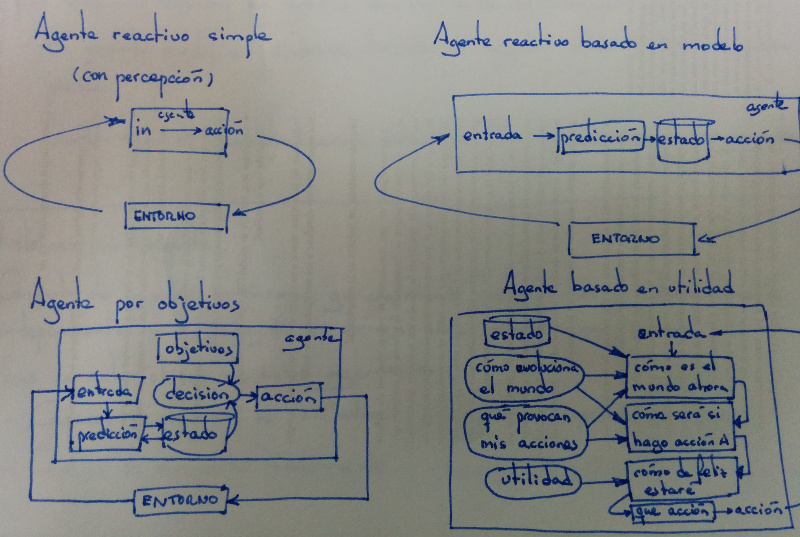
\includegraphics{agent-types}
	\caption[Arquitecturas de agente según su comportamiento]{Distintas arquitecturas de agentes en función del comportamiento. Dependiendo de las acciones a realizar, se identifican tres tipos, los reactivos que aplican una acción sin proceso deductivo y los basados en modelo y utilidad (en algunos contextos denominados deliberativos) que basan su comportamiento en alguna forma de deducción.}
	\label{fig:agent-types}
\end{figure}

La siguiente clasificación viene motivada por la forma de deducir el conjunto de acciones a ser aplicadas por parte de los sensores. En este sentido podemos identificar tres tipos distintos de agentes (figura\ref{fig:agent-types}):

\begin{itemize}
	\item \textbf{Reactivos}. Son aquellos donde el uso de un proceso de razonamiento explícito es demasiado costoso para producir una conducta en un tiempo aceptable. Se suelen implementar como correspondencias (percepción $\rightarrow$ acción) sin ningún razonamiento adicional.
	\item \textbf{Basados en objetivos}. Plantean una deducción de forma que determinan cuál sería el estado del entorno tres aplicar varias o todas las acciones que puede realizar. En base a los resultados, selecciona la acción que se corresponde con sus propios objetivos.
	\item \textbf{Basados en utilidad}. Éstos plantean una deducción similar a los basados en objetivos con la diferencia de que, mientras los primeros sólo diferencian entre entorno objetivo o no objetivo, éstos asignan un valor (i.e. \textit{utilidad}) a cada uno de los escenarios de entorno posibles para seleccionar el mejor (e.g. el que mayor utilidad tiene).
\end{itemize}

En la literatura se describen muchos tipos de agente, como por ejemplo los agentes BDI (Believe-Desire-Intention) o los agentes lógicos (i.e. el entorno se representa con reglas lógicas y se infiere mediante métodos como por ejemplo deducción lógica o prueba de teoremas). Sin embargo, éstos pueden definirse en los términos aquí expuestos (figuras~\ref{fig:agent-basic-architecture}, \ref{fig:memory-vs-amnesia-in-agents} y \ref{fig:agent-types}). 

\subsection{\Glsentrylongsp{mas}}

Son aquellos sistemas compuestos de dos o más agentes que interactúan de alguna manera para llegar a una solución.

Cuando los agentes son inteligentes y el problema cae dentro del dominio de la \gls{ai}, el ámbito de estudio es el de la \gls{dai}, la rama dedicada a la resolución de problemas mediante procesamiento descentralizado.

Desde el punto de vista de la ingeniería de sistemas, y a pesar del aumento de complejidad, los \ac{mas}, al ser sistemas inherentemente descentralizados, ofrecen múltiples ventajas frente a los sistemas centralizados tradicionales:

\begin{itemize}
	\item Los sistemas son más robustos y fiables frente a fallos, ya que los agentes son autónomos e independientes del resto.
	\item La modificación del sistema se puede realizar sobre la marcha, agente a agente sin necesidad de parar el sistema al completo.
	\item Su diseño fuerza a desacoplar las dependencias entre agentes.
	\item Son inherentemente paralelizables y por tanto pueden llegar a ser más eficientes que sus homólogos centralizados. Este punto es quizá el más controvertido, ya que esta ganancia en eficiencia se puede perder rápidamente en función de la cantidad de comunicación existente entre agentes.
	\item Debido al nivel de complejidad alcanzado en los sistemas existentes en la actualidad, la computación se distribuye a través de múltiples sistemas, normalmente heterogéneos. La tendencia además es a la alza. La definición de los \ac{mas} hace natural su implementación en este tipo de arquitecturas.
\end{itemize}
	
Desde el punto de vista de la \gls{ai} podemos añadirles la ventaja de que permiten el estudio de conductas complejas de poblaciones a partir del comportamiento de sus elementos básicos, facilitando el estudio de modelosy de teorías sobre éstos.

\newthought{La comunicación entre agentes}, se trata de una característica clave en un \gls{mas}, ya que para denominarse de esta manera dos o más agentes deben interactuar (i.e. comunicarse) entre si. Esta interacción puede implementarse de diversas maneras\sidenote{Las formas clásicas de comunicación son el de paso de mensajes, los sistemas de pizarra y la estigmergia. Para los dos primeros existen dos propuestas para estándar de lenguaje de comunicación, \Ac{kqml} (\cite{Finin1994}) y \Ac{acl} (\cite{Poslad2007}). La tercera forma de comunicación suele ser muy dependiente del problema y no se apoya en lenguajes estándares. Se trata de una forma de comunicación basada en la modificación del entorno, como la efectuada por las hormigas en la búsqueda de alimento, donde éstas dejan rastros de feromonas modificando el entorno para modificar el comportamiento del resto de la colonia.} y siempre toman una o las dos formas siguientes (figura~\ref{fig:communication-between-agents-in-mass}):

\begin{itemize}
	\item \textbf{Cooperación}. Los agentes intercambian información entre sí para llegar a una solución. Esta solución puede ser fragmentada (i.e. cada agente posee parte de la solución y se comunican para ir avanzando de forma común hacia la solución global) o poseerla uno o varios agentes que hacen uso de más agentes para ir avanzando la solución.
	\item \textbf{Competición}. Los agentes compiten dentro de un entorno, generalmente mediante la adquisición de recursos limitados. Un ejemplo de este tipo de sistemas multiagente puede ser aquellos sistemas de vida artificial.
\end{itemize}

\begin{figure}
	\missingfigure[figheight=3.5cm]{Una ilustración de algún entorno de vida artificial donde los agentes compiten y uno de algo donde cooperen}
	\caption[Diferencias entre colaboración y competitividad de agentes]{La comunicación entre agentes puede ser de dos tipos: \textit{colaborativa}, donde los agentes tratan de llegar a una solución intercambiándose información y \textit{competitiva}, donde los agentes compiten unos contra otros en un entorno.}
	\label{fig:communication-between-agents-in-mass}
\end{figure}
